\section{Experiments}
\label{results}
%From ILO:
%"Plan and carry out a small-scale investigation of an algorithmic research problem. This investigation could be theoretical, experimental, or both."
This sections describes the results reached in the project. The goal in this section is threefold. Firstly to verify the results achieved in \cite{wagner17}. Secondly to explore the performance of \qs{} on new datasets. These datasets will have different properties than the datasets tested in \cite{wagner17}. Lastly to discover the performance of \qsr{} and compare this to the performance of \qs{}. 
\\
\\
The expirements are based on two datasets from the paper as well as two new datasets.\footnote{From \cite{wagner17} we use the datasets \sift{} and \mnist{}. Explicitly in this paper we have included \clust{} and \gist{}} For each dataset the results of \qs{} is verified and compared to the baseline implementation \gr{} and to \qsr{}. 
\\
\\
The results of these tests are illustrated as line charts. The charts visualizes the performance of the algorithms for each dataset measured in terms of \textit{accuracy pr bit of precision} and \textit{distortion pr bit of precision}. 
\\
\\
Similarly as in \cite{wagner17} the \qs{} implementations has been parameterized with \textit{L} ranging from 2 till 10 and $\Lambda$ ranging from \textit{L$_{min}$-1} to \textit{L$_{max}$-1}.\footnote{Their experiments range from \textit{L} ranging from 2 till 20 and $\Lambda$ 1 till 19. However the computation time for trees with a depth $>$ 14 is immense.} 
%\subsection{Practical improvements}
%Instead of randomly shifted ( works well for arbitrary, but maybe we know our data )
%On specific datasets:
%- Scale on spread out datasets, to avoid one point in each quad leaf
%- Zoom in on narrow / close datasets
\\
\\
The charts presented below displays results from the dataset \sift{}, \mnist{}. These results are key in verifying the results presented in \cite{wagner17}. Following this are the charts displaying results from \clust{} and \gist{}, as these disclose new information about the overall performance of \qs{}. Two graphs exists for each dataset displaying \textit{accuracy} and \textit{distortion} respectively. The graphs display that \qs{} has a better performance than \grid{} and verifies the results presented from empirical experiments in \cite{wagner17}.

\begin{figure}[h!]
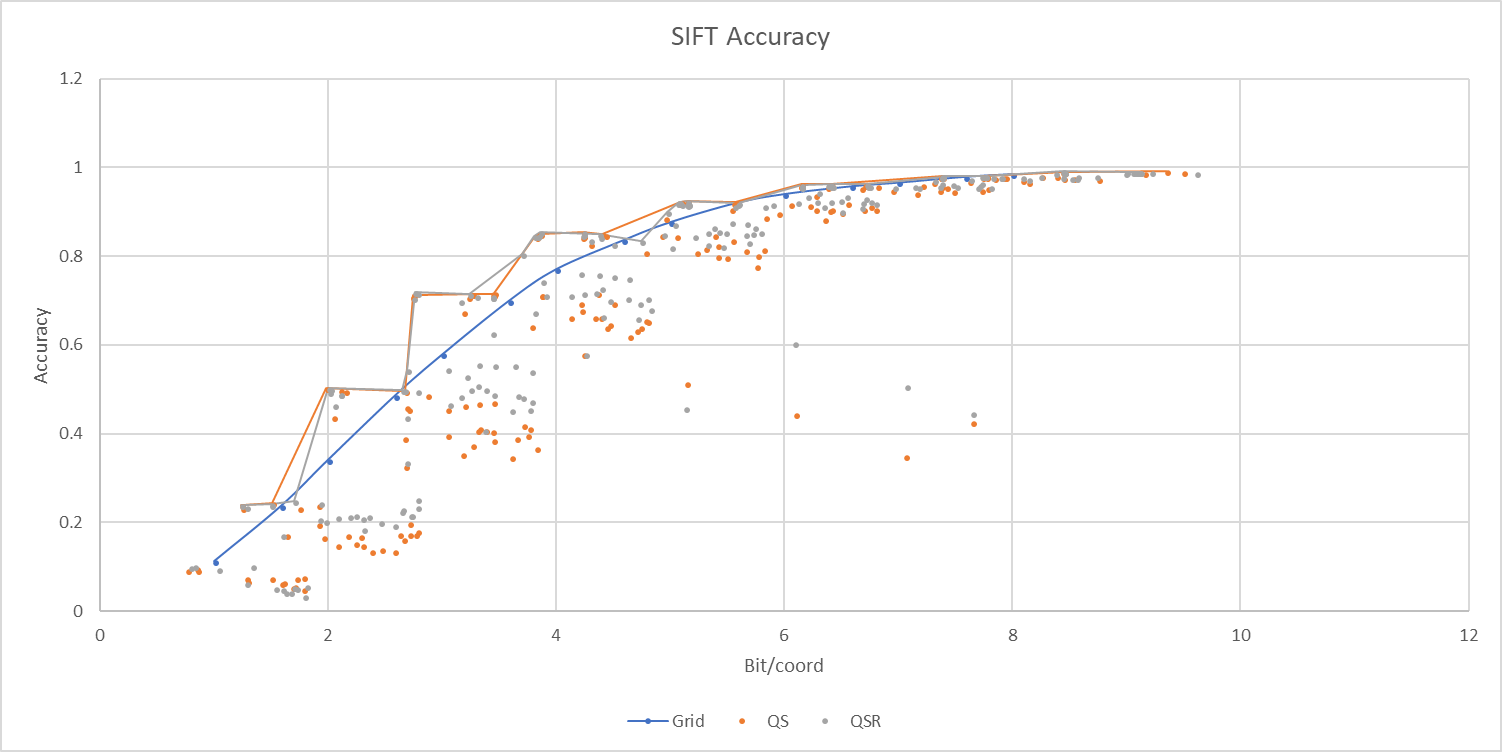
\includegraphics[width=\textwidth]{figures/graphs/sift_accuracy}
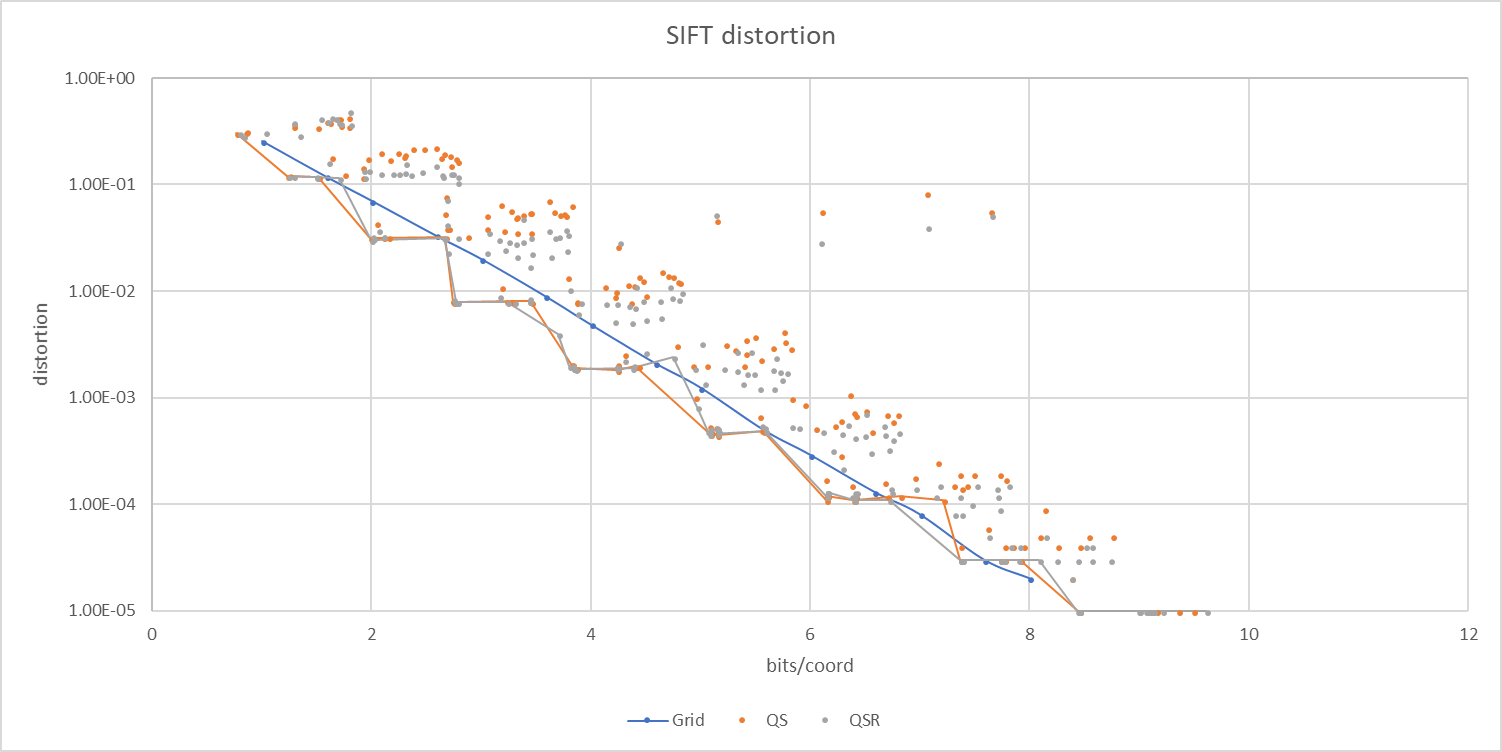
\includegraphics[width=\textwidth]{figures/graphs/sift_distortion}
\caption{Accuracy and distortion from \sift{}}
\label{fig:graph sift}
\end{figure}
The graphs in figure \ref{fig:graph sift} above show that in the best case scenario for \qs{} and \qsr{} are quite similar, while \qsr{} seems to be better in the average case.

\begin{figure}[h!]
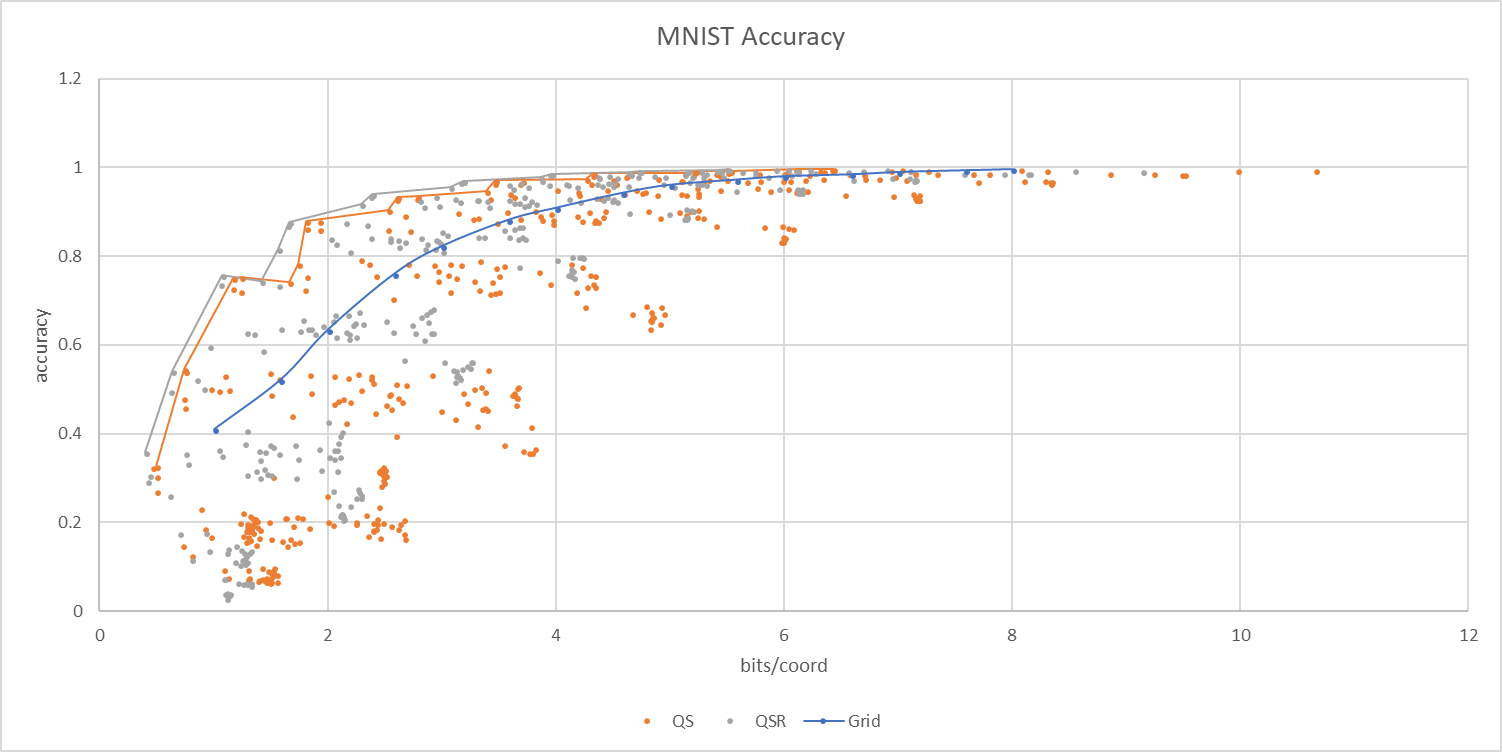
\includegraphics[width=\textwidth]{figures/graphs/mnist_accuracy}
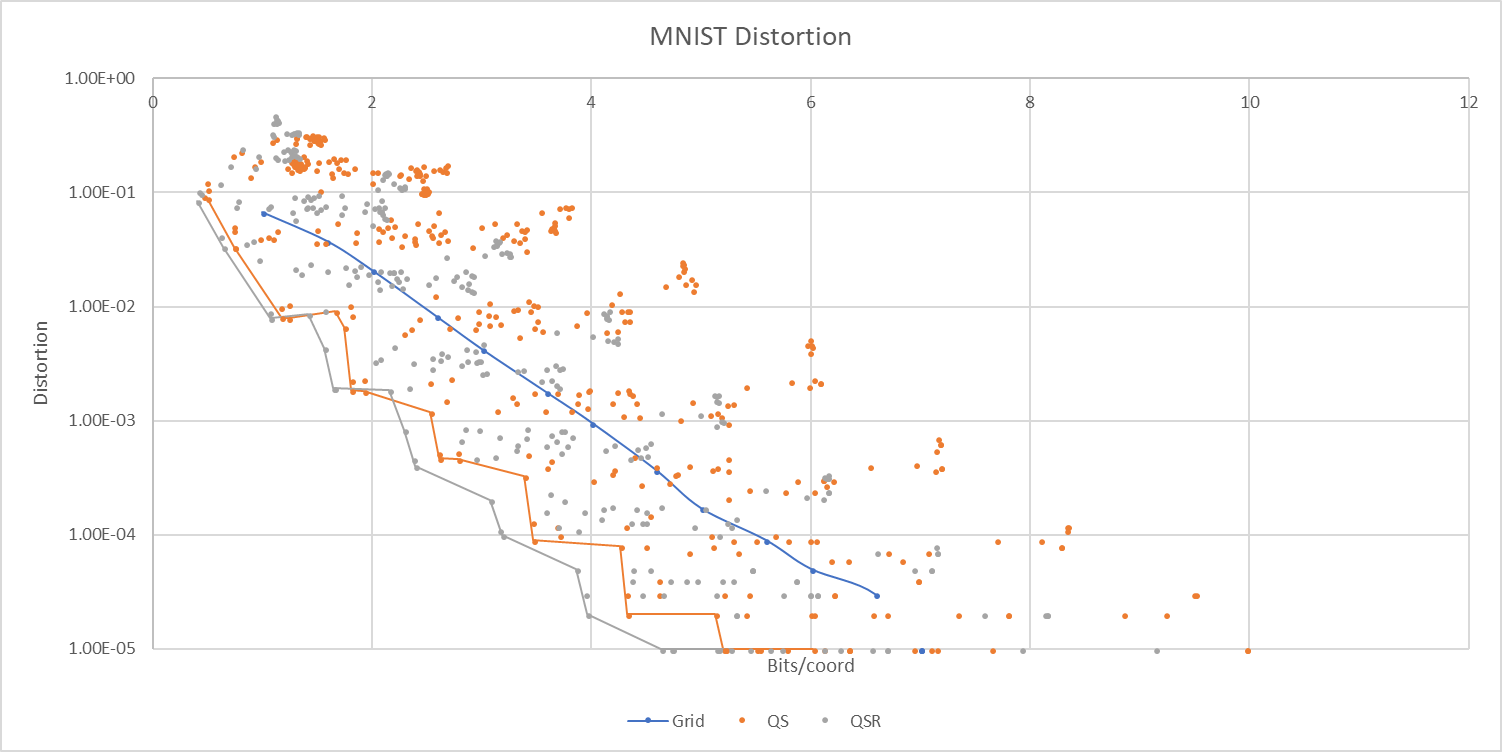
\includegraphics[width=\textwidth]{figures/graphs/mnist_distortion}
\caption{Accuracy and distortion from \mnist{}}
\label{fig:graph mnist}
\end{figure}
\clearpage
Figure \ref{fig:graph mnist} displays that \qsr{} runs are slightly superior to \qs{} in the best case regarding accuracy, and superior in regards to distortion. The average case for \qsr{} in distortion seems superior to the average case in \qs{}, but similar in regards to accuracy.

\begin{figure}[h!]
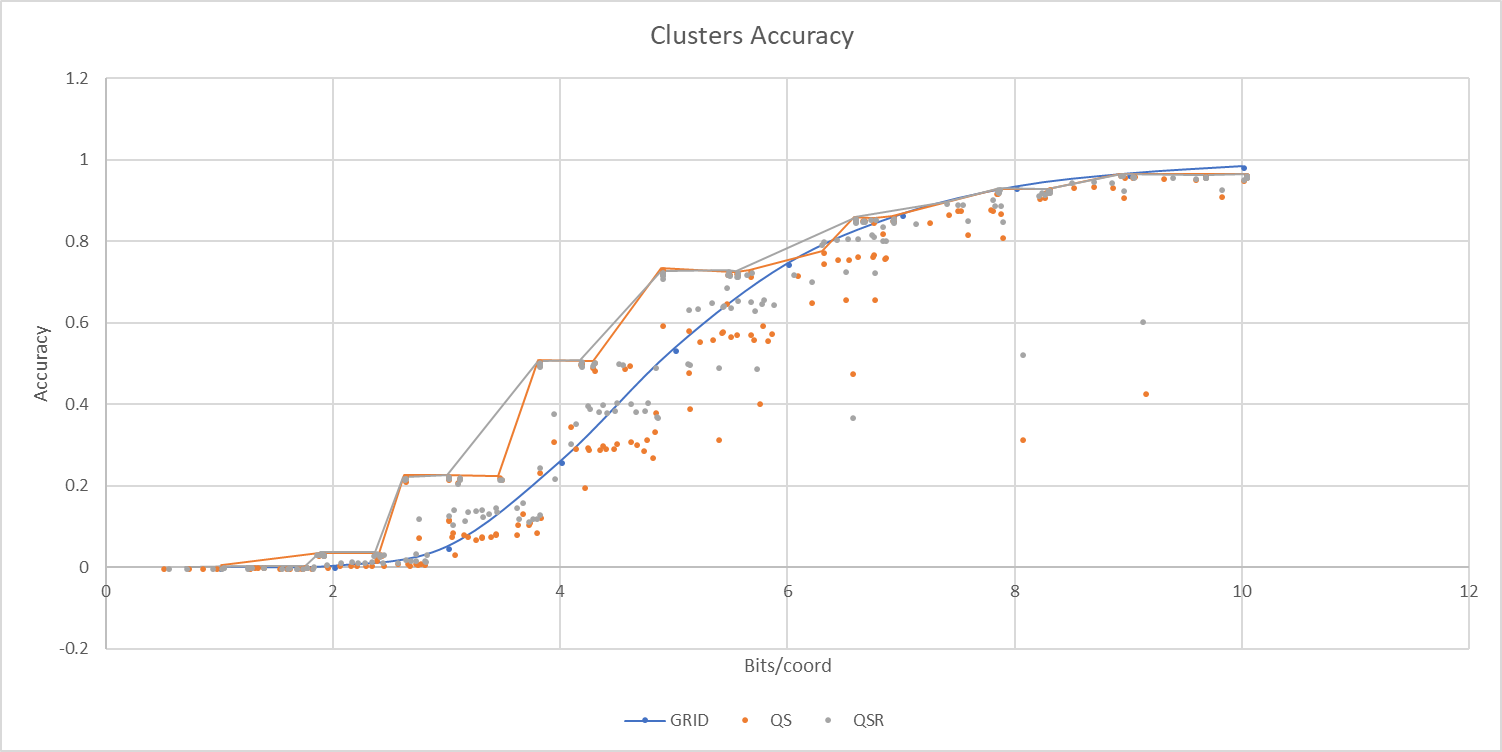
\includegraphics[width=\textwidth]{figures/graphs/clusters_accuracy}
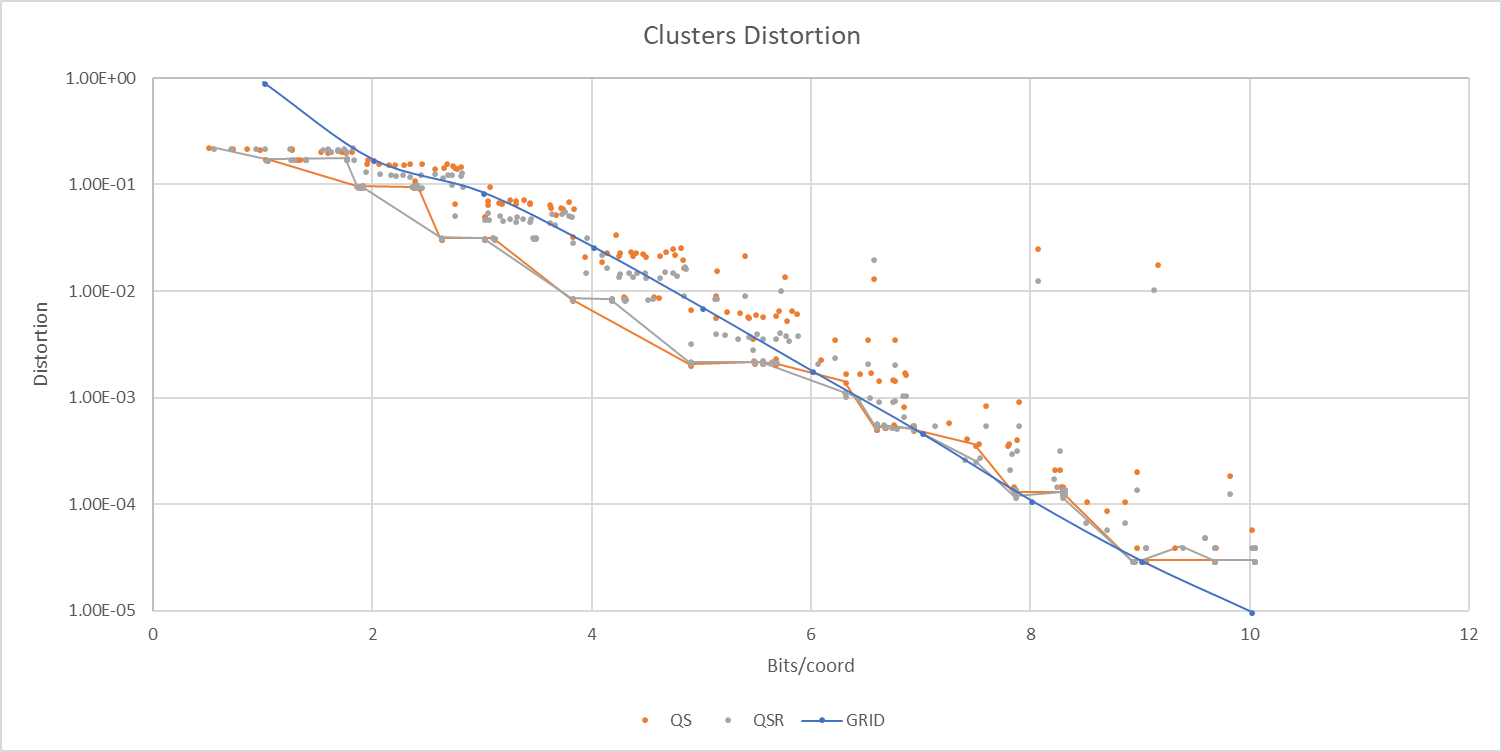
\includegraphics[width=\textwidth]{figures/graphs/clusters_distortion}
\caption{Accuracy and distortion from \clust{}}
\label{fig:graph clust}
\end{figure}
Figure \ref{fig:graph clust} shows that \qs{} and \qsr{} behaves similarly in best case runs for the clusters dataset. However the average case for \qsr{} is slightly superior to the \qs{} average results both regarding accuracy and distortion.
\clearpage{}

%\begin{figure}[h]
%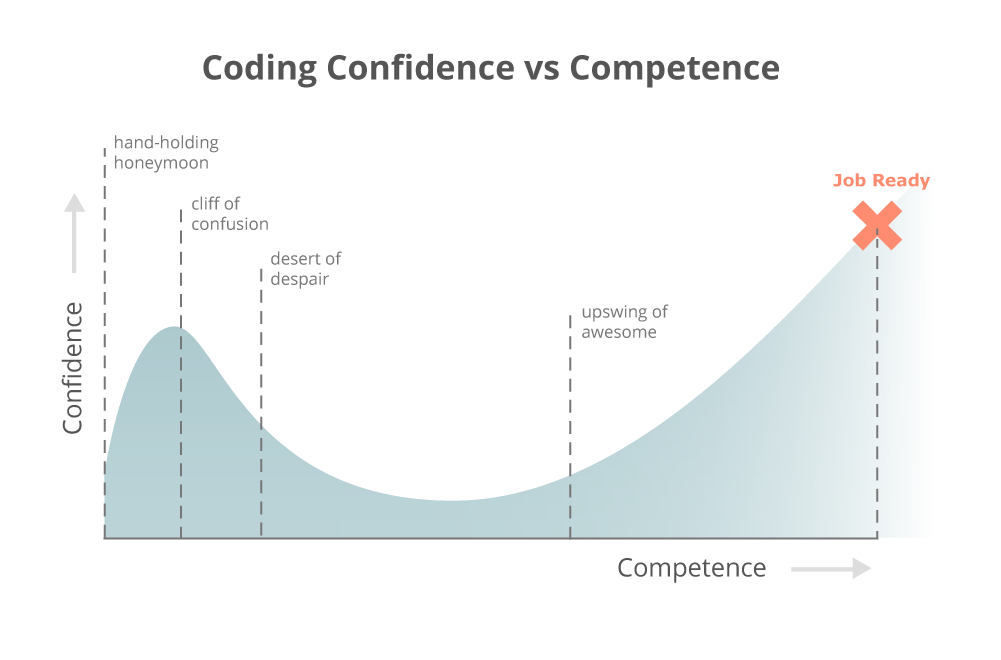
\includegraphics[width=0.5\textwidth]{figures/coding_graph}
%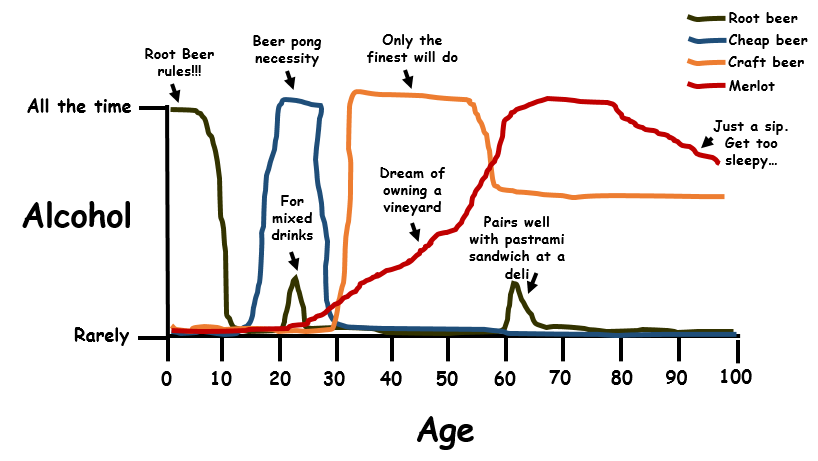
\includegraphics[width=0.5\textwidth]{figures/alcohol_graph}
%\caption{Accuracy and distortion from \gist{}}
%\label{fig:graph gist}
%\end{figure}

\begin{table}[h]
	\centering
	\caption{Average Results for \qs{} on \mnist{}}
	\label{table:avg_mnist_qs2}
	\begin{tabular}{l l l l}
		\hline
		\#Blocks & Bits per coordinate & Accuracy  & Distortion \\ \hline
		2 & 3.43 & 0.44 & 1.100  \\
		4 & 4.36 & 0.51 & 1.096  \\
		7 & 3.75 & 0.53 & 1.097 \\
		8 & 3.69 & 0.56 & 1.09 \\
		14 & 3.51 & 0.67 & 1.048 \\
		16 & 3.45 & 0.69 & 1.039 \\
		28 & 3.35 & 0.81 & 1.013 \\
		\hline
	\end{tabular}
\end{table}

\begin{table}[h]
	\centering
	\caption{Average Results for \qsr{} on  \mnist{}}
	\label{table:avg_mnist_qsr2}
	\begin{tabular}{l l l l}
		\hline
		\#Blocks & Bits per coordinate & Accuracy  & Distortion \\ \hline
		2 & 3.79 & 0.55 & 1.118  \\
		4 & 3.73 & 0.57 & 1.09  \\
		7 & 3.21 & 0.62 & 1.062 \\
		8 & 3.16 & 0.64 & 1.052 \\
		14 & 3.01 & 0.74 & 1.023 \\
		16 & 2.95 & 0.76 & 1.02 \\
		28 & 2.87 & 0.85 & 1.008 \\
		\hline
	\end{tabular}
\end{table}


\begin{table}[h!]
	\centering
	\caption{Average Results for \qs{} on \sift{}}
	\label{table:avg_sift_qs}
	\begin{tabular}{l l l l}
		\hline
		\#Blocks & Bits per coordinate & Accuracy  & Distortion \\ \hline
		2 & 4.32 & 0.49 & 1.122  \\
		4 & 4.64 & 0.61 & 1.056  \\
		8 & 4.39 & 0.7 & 1.034 \\
		16 & 5.15 & 0.85 & 1.008 \\
		32 & 5.68 & 0.78 & 1.025 \\
		\hline
	\end{tabular}
\end{table}

\begin{table}[h!]
	\centering
	\caption{Average Results for \qsr{} \sift{}}
	\label{table:avg_sift_qsr}
	\begin{tabular}{l l l l}
		\hline
		\#Blocks & Bits per coordinate & Accuracy  & Distortion \\ \hline
		2 & 4.33 & 0.52 & 1.112  \\
		4 & 4.63 & 0.65 & 1.04  \\
		8 & 5.02 & 0.77 & 1.018 \\
		16 & 5.44 & 0.83 & 1.015 \\
		32 & 5.68 & 0.79 & 1.02 \\
		\hline
	\end{tabular}
\end{table}

\begin{table}[h!]
	\centering
	\caption{Average Results for \qs{} \clust{}}
	\label{table:avg_clust_qs}	
	\begin{tabular}{l l l l}
		\hline
		\#Blocks & Bits per coordinate & Accuracy  & Distortion \\ \hline
		2 & 4.27	& 0.32 & 1.085  \\
		4 & 4.51 & 0.39 & 1.058  \\
		8 & 4.97 & 0.49 & 1.034 \\
		16 & 5.72 & 0.59 & 1.026 \\
		32 & 5.75 & 0.57 & 1.036 \\
		\hline
	\end{tabular}
\end{table}

\begin{table}[h!]
	\centering
	\caption{Average Results for \qsr{} on \clust{}}
	\label{table:avg_clust_qsr}
	\begin{tabular}{l l l l}
		\hline
		\#Blocks & Bits per coordinate & Accuracy  & Distortion \\ \hline
		2 & 4.26 & 0.33 & 1.08  \\
		4 & 4.5 & 0.42 & 1.048  \\
		8 & 4.97 & 0.52 & 1.03 \\
		16 & 5.72 & 0.61 & 1.025 \\
		32 & 6.08 & 0.63 & 1.026 \\
		\hline
	\end{tabular}
\end{table}
